\documentclass[tikz]{standalone}
\begin{document}

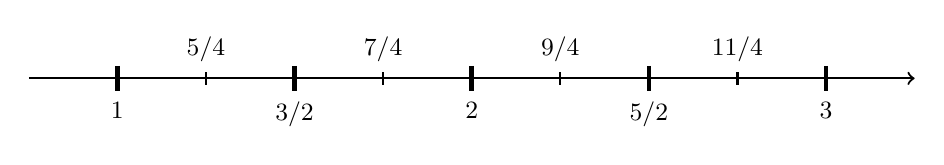
\begin{tikzpicture}[baseline=-0.5ex,scale=4.5]
  \draw[thick,->] (0.75,0) -- (3.25,0);
  \foreach \x in {1, 2, 3}{
    \draw [ultra thick] (\x cm,1.0pt) -- (\x cm,-1.0pt) node[below]{\small$\x$};
  }
  \foreach \x in {3, 5}{
    \draw [ultra thick] (0.5*\x cm,1.0pt) -- (0.5*\x cm,-1.0pt) node[below]{\small$\x/2$};
  }
  \foreach \x in {5, 7,9,11}{
    \draw [thick] (0.25*\x cm,-0.5pt) -- (0.25*\x cm,0.5pt) node[above]{\small$\x/4$};
  }
\end{tikzpicture}
\end{document} 
